\documentclass{article}
\usepackage[a4paper, margin=1.5cm]{geometry}
\usepackage{graphicx}
\usepackage{hyperref}
\usepackage{amsmath}
\usepackage{siunitx}

\title{DARES Electronics: BMS and Power Systems \\
Mid-semester Break Plan}

\author{Prepared by (Alfred) Zi Wang}
\date{September 2026}

\begin{document}

\maketitle

\section{System Overview}

The power system is responsible for safely storing, distributing, monitoring, and supplying electrical energy to every subsystem on the drone.

\begin{figure}[h]
    \centering
    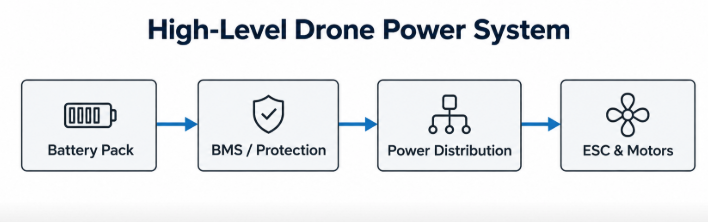
\includegraphics[width=1\linewidth]{Power.png}
    \caption{High level block diagram}
\end{figure}


with additional regulated outputs supplying:

\begin{center}
Flight Controller, Sensors, Communications, Navigation Electronics, and Other Low-Power Loads.
\end{center}


\section{Our Main Design Questions}

\begin{itemize}

\item \textbf{What battery should we use?}

We need to determine the required battery voltage, capacity, discharge rate, mass, and chemistry based on the propulsion system, flight controller and expected flight time.  Also check the input constraints (voltage, current) of the flight controller or power distribution board.

\item \textbf{How much current does the drone require?}

The motor and ESC will dominate the power consumption. We need to estimate both continuous current and short-duration peak current.

\item \textbf{How do we safely monitor the battery?}

The system should measure important quantities such as:
\begin{itemize}
    \item Battery voltage
    \item Individual cell voltages
    \item Battery current
    \item Battery temperature
    \item State of Charge (SOC) \\
    (Percentage of usable battery capacity remaining, e.g. 100\%, 50\%)
\end{itemize}

\item \textbf{What protection do we need?}

Possible protection functions include:
\begin{itemize}
    \item Over-voltage protection
    \item Under-voltage protection
    \item Over-current protection
    \item Short-circuit protection
    \item Over-temperature protection
    \item Cell balancing
\end{itemize}

\item \textbf{How should power be distributed?}

We need to determine how the battery connects to:
\begin{itemize}
    \item ESCs and motors
    \item Flight controller
    \item Sensors
    \item Radio / telemetry
    \item Navigation electronics
    \item Payload electronics
\end{itemize}


\end{itemize}


\section{General Design Process}

\begin{itemize}

\item Start by determining the expected electrical requirements of each subsystem.

\item Create a \textbf{power budget} containing:
\begin{itemize}
    \item Operating voltage
    \item Average current
    \item Peak current
    \item Average power
    \item Maximum power
\end{itemize}

\item Use propulsion data to estimate the maximum battery current.

\item Select a battery voltage and capacity that satisfy the propulsion requirements and expected flight duration.

\item Determine suitable connectors, cables, PCB traces, fuses, switches, and power distribution hardware based on the expected maximum current.

\item Design the low-voltage power supplies required by the electronics.

\item Implement battery manage system for voltage, current, and temperature monitoring, protection and, if required, cell balancing.

\item Test each subsystem individually before integrating the complete drone.

\end{itemize}

\section{Battery Management System}

The Battery Management System (BMS) monitors the condition of the battery and helps protect it from unsafe operating conditions.

A simplified BMS structure may include:

\begin{figure}[h]
    \centering
    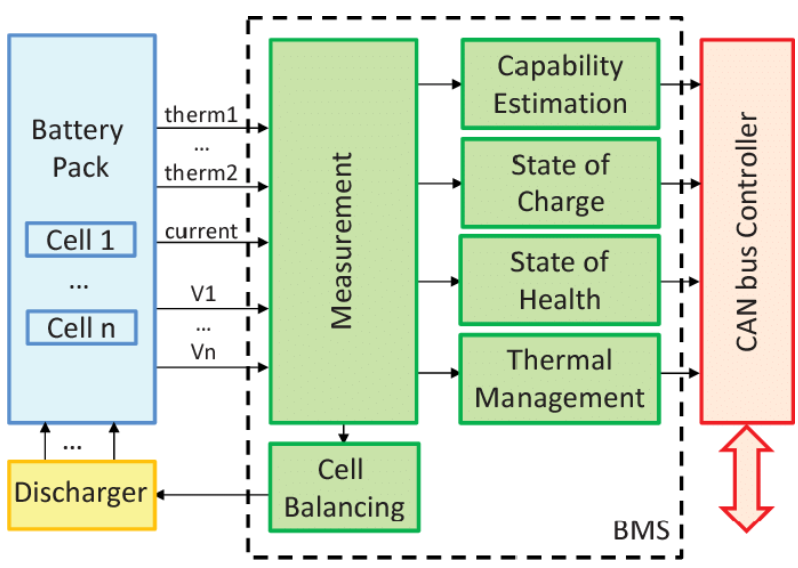
\includegraphics[width=1\linewidth]{BMS.png}
    \caption{BMS block diagram}
\end{figure}

\newpage

\section{Power Distribution System}
The power is then divided into two main branches:

\begin{figure}[h]
    \centering
    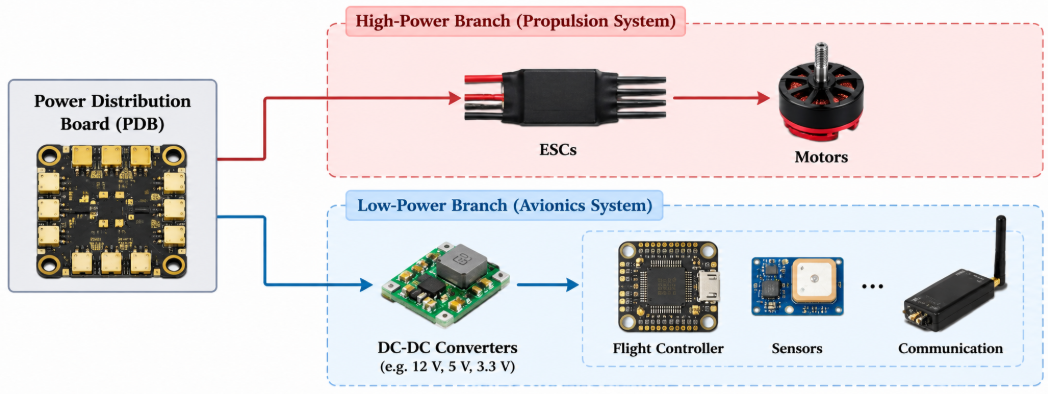
\includegraphics[width=1\linewidth]{PDB.png}
    \caption{Power Distribution diagram}
\end{figure}

\begin{itemize}

\item \textbf{High-Power Branch}

Supplies the propulsion system:

This branch carries the largest current in the drone and therefore requires appropriately rated connectors, wires, PCB copper, and protection devices.

\item \textbf{Low-Power Branch}

Supplies the control and sensing electronics:

\begin{center}
Power Distribution Board
$\rightarrow$
DC--DC Converters
$\rightarrow$
Flight Controller / Sensors / Communication
\end{center}

The battery voltage is converted into regulated voltage rails such as
\SI{12}{V}, \SI{5}{V}, or \SI{3.3}{V}, depending on the requirements of the electronics.

\end{itemize}

\newpage

\section{Software}

The following tools will likely be useful:

\begin{itemize}

\item \textbf{MATLAB / Python}

For:
\begin{itemize}
    \item Battery data analysis
    \item Flight-time estimation
    \item Power-budget calculations
    \item SOC algorithm development
\end{itemize}

\item \textbf{LTspice}

For:\\
Circuit design and analysis
\begin{itemize}
    \item DC--DC converter simulation
    \item Voltage measurement circuits
    \item Current-sensing circuits
    \item Protection circuitry
\end{itemize}

\item \textbf{Cadence}

For:
\begin{itemize}
    \item Schematic design
    \item PCB design
    \item Power distribution board development
    \item Custom BMS PCB development
\end{itemize}

\item \textbf{C / C++}

For implementing battery monitoring and protection logic on the microcontroller.

\end{itemize}



\section{To-Do Over Mid-Semester Break}

The goal over the mid-semester is to understand the basic of drone power system and BMS rather than immediately designing a complete BMS and power distribution.

By the end of mid-semester, each member should watch the videos below and have a basic understanding of:

\begin{itemize}

    \item \textbf{Series and parallel battery connections}

    \href{https://www.youtube.com/watch?v=L-UfAeyTI9g}
    {Series and Parallel Battery Connections}

    \item \textbf{Battery capacity, energy, and C-rating}

    \href{https://www.youtube.com/watch?v=cxkVxi9P0EA}
    {Battery Capacity and Energy}

    \href{https://www.youtube.com/watch?v=5JZ8E7B4FAY}
    {Battery C-Rating}

    \item \textbf{What is a Battery Management System (BMS)?}

    \href{https://www.youtube.com/watch?v=q4wDa_m9-8E}
    {Introduction to Battery Management Systems}

    \href{https://www.youtube.com/watch?v=rT-1gvkFj60}
    {Battery Management System Overview}

    \item \textbf{BMS active and passive cell balancing}

    \href{https://www.youtube.com/watch?v=GXYJ1xC10j4}
    {Active and Passive Cell Balancing}

    \item \textbf{Drone power distribution board explained}

    \href{https://www.youtube.com/watch?v=CU4Tl4xxuh8}
    { Explains Power distribution boards for quadcopter drones}
\end{itemize}

\section{Optional Advanced Research}

For anyone interested in going further, useful topics include:

\begin{itemize}
\item State-of-Charge estimation

\item Equivalent circuit battery models

\item SOC estimation

\item Passive versus active cell balancing

\item Power distribution PCB design

\item CAN-based battery communication

\end{itemize}



\end{document}

